\section{Stability Analysis}\label{sec:stability}
The statements below concern unsaturated, noise-free linear loops. They do not transfer automatically to the saturated nonlinear simulation.

For LQR the uncertain scalar characteristic equation is
\begin{equation}
z-[A_d(C_{\rm th},UA)-B_d(C_{\rm th},UA)K]=0. \label{eq:lqrchar}
\end{equation}
On the continuous box $C_{\rm th}\in[0.7,1.3]C_0$, $UA\in[0.7,1.3]UA_0$, monotonic exponential bounds give intervals for $A_d$ and $B_d$. Natural interval evaluation of \cref{eq:lqrchar} leaves a positive unit-circle margin 0.003961, formally certifying the original LQR for this box.

The LQI closed-loop matrix is
\begin{equation}
F_{\rm LQI}=\begin{bmatrix}A_d-B_dK_x&-B_dK_z\\-h&1\end{bmatrix}. \label{eq:lqimatrix}
\end{equation}
For characteristic polynomial $z^2-tz+\delta$, second-order Jury conditions are $1-t+\delta>0$, $1+t+\delta>0$, and $1-\delta>0$. Validated outward-conservative interval evaluation over $128^2$ covering subboxes gives minimum margins $3.19\times10^{-5}$, 3.95, and 0.0137, respectively. Their positivity certifies original LQI stability throughout the continuous box; subdivision only reduces dependency overestimation and does not omit points.

The implemented PID has a fourth-order linear realization because integral, filtered derivative, and previous measurement are states. Its characteristic equation is $\det(zI-F_{\rm PID})=0$, where $F_{\rm PID}$ is generated directly from the discrete update. A 61-by-61 grid gives spectral radius 0.992397--0.995996, but coefficient dependencies prevent the present interval calculation from proving the full box. Formal PID robust stability therefore remains unproven.
\begin{table}[!htbp]\centering\caption{Formal and gridded stability evidence.}\label{tab:stability}\resizebox{\linewidth}{!}{\begin{tabular}{lcc}\toprule
Controller & Formal interval result & Grid radius range \\
\midrule
PID & Unproven & 0.992397--0.995996 \\
LQR & Certified (margin 0.003961) & 0.991930--0.996039 \\
LQI & Certified (min. Jury margin 0.000032) & 0.986843--0.993128 \\
\bottomrule\end{tabular}
}\end{table}
\begin{figure}[t]\centering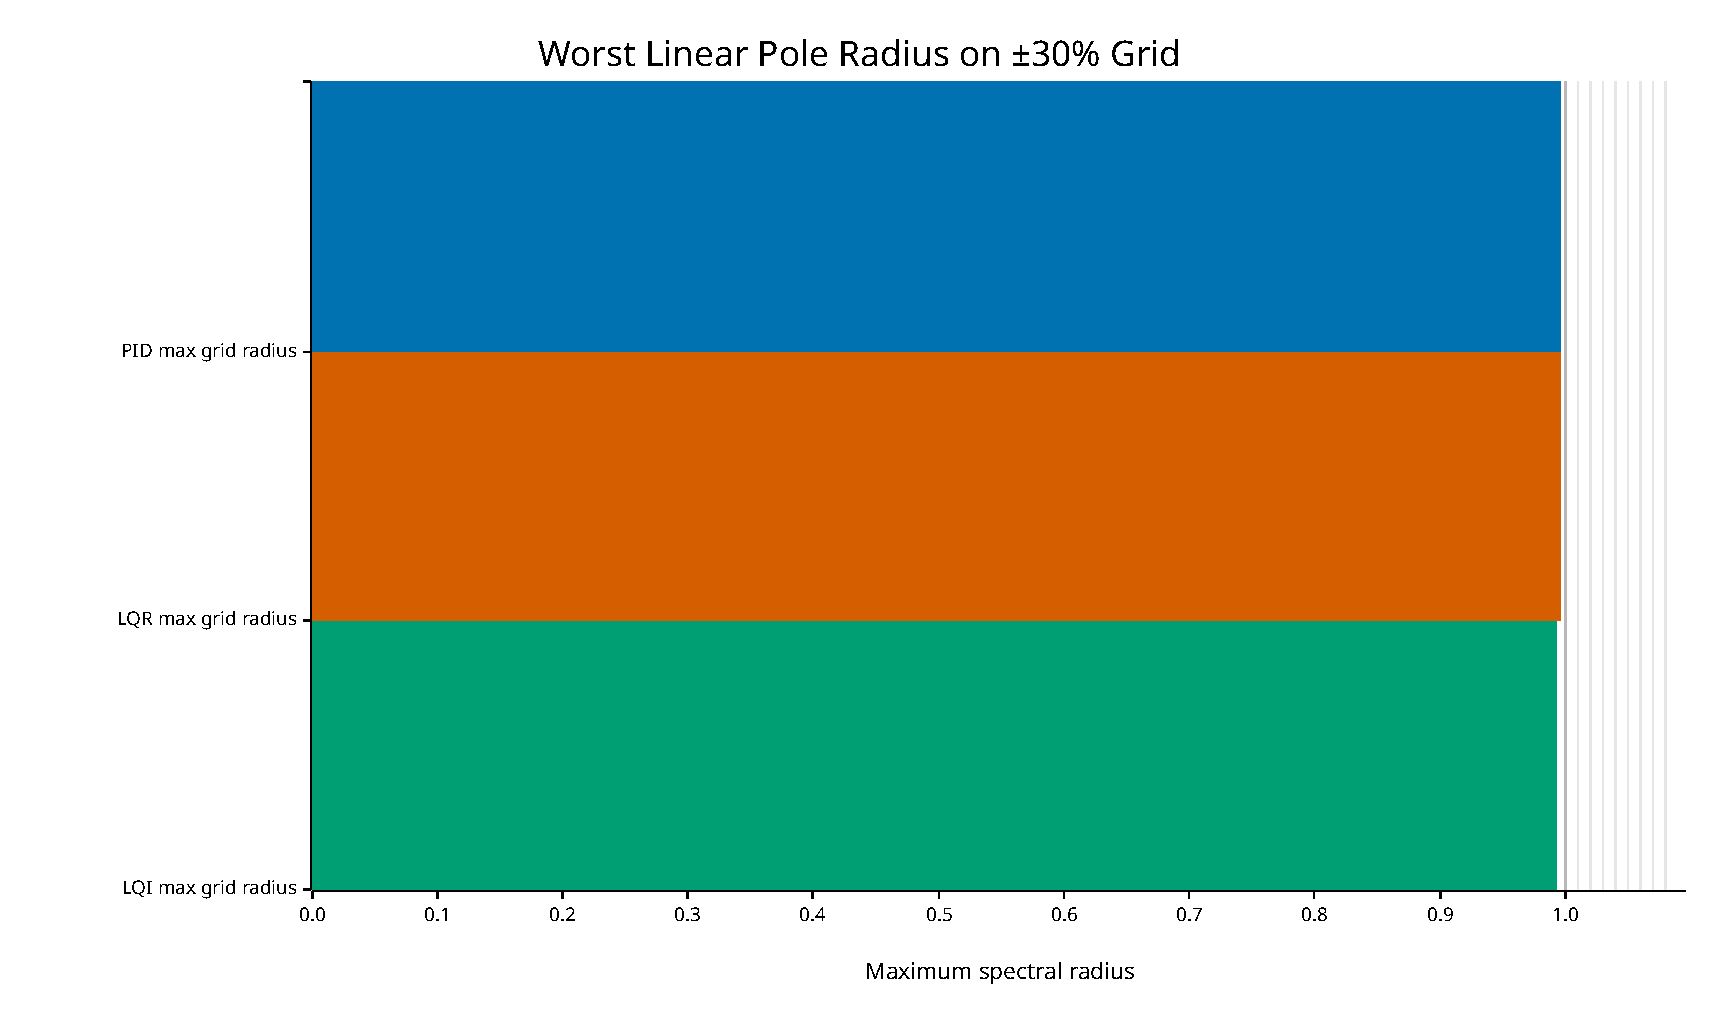
\includegraphics[width=\linewidth]{figures/stability-domain-summary.pdf}\caption{Worst spectral radius on the integer uncertainty grid. This figure is supporting numerical evidence, not the interval proof.}\label{fig:stability}\end{figure}
\FloatBarrier

